\documentclass[12pt,letterpaper]{article}
\usepackage[utf8]{inputenc}
\usepackage[spanish]{babel}
\usepackage{graphicx}
\usepackage[left=2cm,right=2cm,top=2cm,bottom=2cm]{geometry}
\usepackage{graphicx} % figuras
% \usepackage{subfigure} % subfiguras
\usepackage{float} % para usar [H]
\usepackage{amsmath}
%\usepackage{txfonts}
\usepackage{stackrel} 
\usepackage{multirow}
\usepackage{enumerate} % enumerados
\renewcommand{\labelitemi}{$-$}
\renewcommand{\labelitemii}{$\cdot$}
% \author{}
% \title{Caratula}
\begin{document}

% Fancy Header and Footer
% \usepackage{fancyhdr}
% \pagestyle{fancy}
% \cfoot{}
% \rfoot{\thepage}
%

% \usepackage[hidelinks]{hyperref} % CREA HYPERVINCULOS EN INDICE

% \author{}
\title{Caratula}

\begin{titlepage}
\begin{center}
\large{UNIVERSIDAD PRIVADA DE TACNA}\\
\vspace*{-0.025in}
\begin{figure}[htb]
\begin{center}
\vspace{\baselineskip}

\includegraphics[width=4.5cm]{./Imagenes/logo}
\end{center}
\end{figure}
\vspace*{0.15in}
INGENIERIA DE SISTEMAS  \\

\vspace*{0.5in}
\begin{large}
TITULO:\\
\end{large}

\vspace*{0.1in}
\begin{Large}
\textbf{INFORME DE LABORATORIOS} \\
\end{Large}

\vspace*{0.3in}
\begin{Large}
\textbf{CURSO:} \\
\end{Large}

\vspace*{0.1in}
\begin{large}
BASE DE DATOS II\\
\end{large}

\vspace*{0.3in}
\begin{Large}
\textbf{DOCENTE:} \\
\end{Large}

\vspace*{0.1in}
\begin{large}
 ING. Patrick Cuadros Quiroga\\
\end{large}

\vspace*{0.2in}
\vspace*{0.1in}
\begin{large}
Integrantes: \\
\vspace{\baselineskip}
\begin{flushleft}
Condori Gutierrez, Flor de Maria            	\hfill	(2015053227) \\
Escalante Maron,  Nelia            	\hfill	(2014049551) \\
Salamanca Contreras, Fiorella Rosmery           	\hfill	(2015053237) \\
\end{flushleft}
\end{large}
\end{center}

\end{titlepage}

\tableofcontents % INDICE
\thispagestyle{empty} % INDICE SIN NUMERO
\newpage
\setcounter{page}{1} % REINICIAR CONTADOR DE PAGINAS DESPUES DEL INDICE

\section{Pasos previo a la instalacion de la Maquina Virtual OEL 6.6} 
 Como primer paso vamos a crear la carpeta en la siguiente ubicación en el Disco Local E con el nombre de “VMs”;
	\begin{center}
		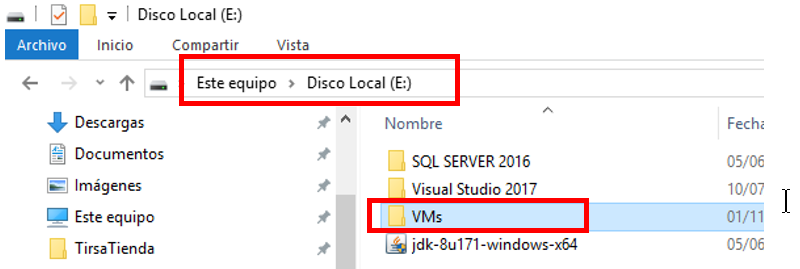
\includegraphics[width=12cm]{./Imagenes/1} 
	\end{center}

\vspace{\baselineskip}
\vspace{\baselineskip}

 Dentro de la carpeta de “VMs” creamos una nueva carpeta con el nombre de “VHDs” donde pasaremos a copiar el archivo de “OEL 6.6”
 	\begin{center}
 		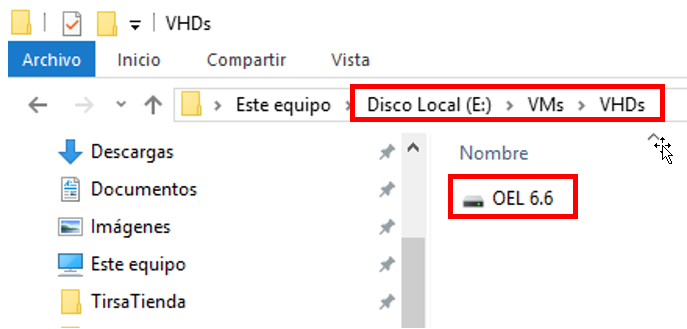
\includegraphics[width=12cm]{./Imagenes/2} 
 	\end{center}
 
 \vspace{\baselineskip}
 
 EN CASO DE NO TENER ACTIVO EL HYPER V: 
 Ingresamos al panel de control dentro de panel de control nos dirigimos hacia la opción de “Programas” 
  	\begin{center}
 	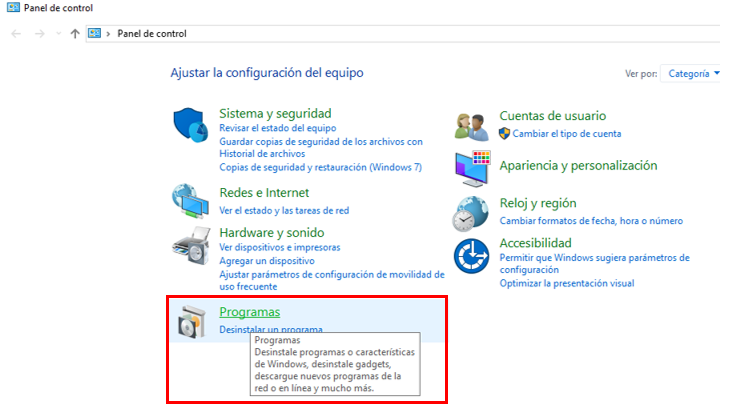
\includegraphics[width=12cm]{./Imagenes/3} 
 	\end{center}
 
 \vspace{\baselineskip}
 
 Dentro escogemos la opción de “Activar o desactivar las características de Windows”
   	\begin{center}
 	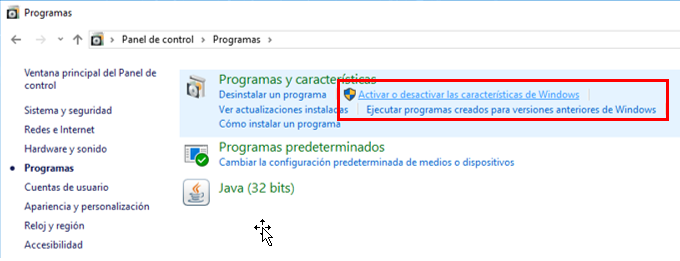
\includegraphics[width=15cm]{./Imagenes/4} 
 	\end{center}
 
 \vspace{\baselineskip}
 
 Buscamos la opción en la que aparece el “Hyper – v” y le damos click y damos “Aceptar”.
    \begin{center}
 	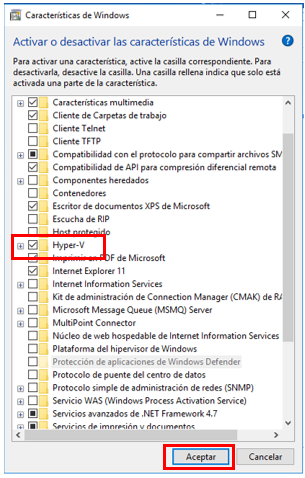
\includegraphics[width=10cm]{./Imagenes/5} 
    \end{center}

\vspace{\baselineskip}

 Al dar aceptar veremos una pantalla que dirá aplicando cambios, esperamos.
     \begin{center}
 	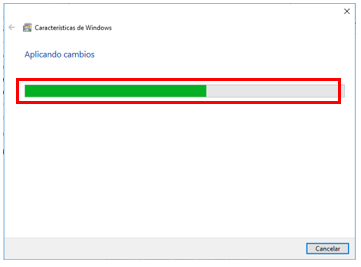
\includegraphics[width=9cm]{./Imagenes/6} 
 	\end{center}
 
 \vspace{\baselineskip}
 
 Al completar los cambios que nos pidió, nos pedirá que reiniciemos el equipo, damos clic en “Reiniciar ahora”, y esperaremos a que se encienda de nuevo nuestro pc.
    \begin{center}
 	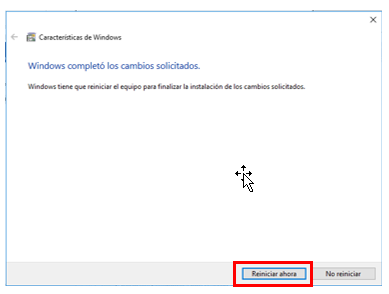
\includegraphics[width=9cm]{./Imagenes/7} 
    \end{center}

Cuando la pc inicie vamos a Windows y en el buscador escribimos “Administrador de hyper-v”, veremos que nos sale la imagen y damos clic a la imagen. 
\begin{center}
	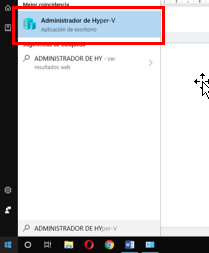
\includegraphics[width=5cm]{./Imagenes/8} 
\end{center}

\vspace{\baselineskip}

Nos mostrara una pantalla del administrador del hyper-v y en donde realizaremos varias acciones. 
\begin{center}
	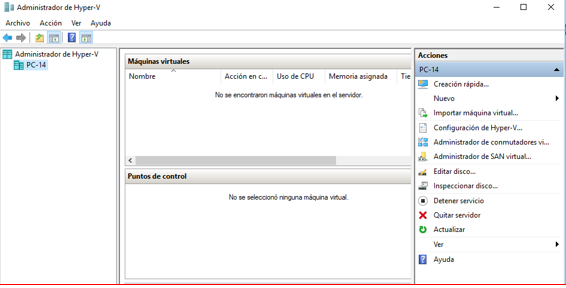
\includegraphics[width=16cm]{./Imagenes/9} 
\end{center}

\vspace{\baselineskip}
\vspace{\baselineskip}

Primero “Examinaremos” y verificaremos la carpeta en donde anteriormente copiamos el archivo de OEL 6.6 escogemos esa carpeta. 
\\
En este parte escogemos la segunda carpeta que hemos creado dentro de VMs, en donde ira la configuración y damos clic en “Aceptar”. 
\begin{center}
	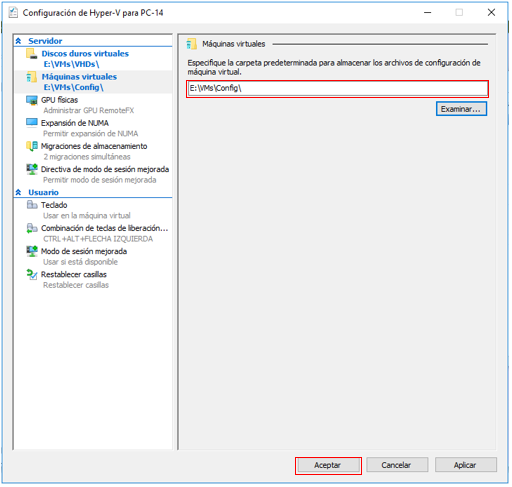
\includegraphics[width=10cm]{./Imagenes/10} 
\end{center}

\newpage

Nos dirigimos hacia “Administrador de conmutadores virtuales”. 
\begin{center}
	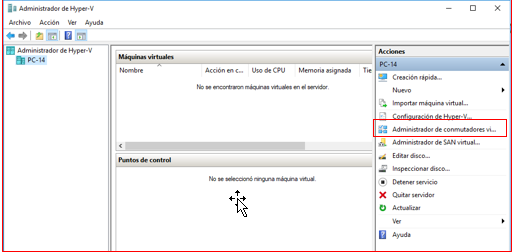
\includegraphics[width=17cm]{./Imagenes/11} 
\end{center}

\vspace{\baselineskip}

Nos mostrarà esta ventana nos preguntara que tenemos que elegir cual conmutador escoger, escogemos el conmutador “Interno”. Y damos clic en “Crear conmutador virtual”.
\begin{center}
	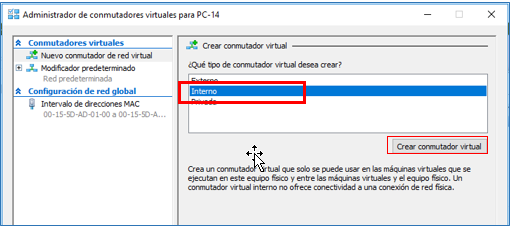
\includegraphics[width=14cm]{./Imagenes/12} 
\end{center} 

\vspace{\baselineskip}

Al crear el conmutador virtual nos pedirá que ingresemos un nombre el que deseemos, en este caso le pondremos de nombre “AdaptadorOracle”, en el tipo de conexión verificaremos que este en “Red interna” y damos clic en “Aceptar”. 
	\begin{center}
		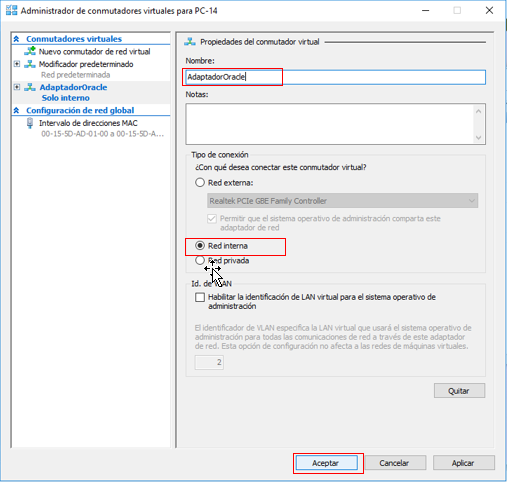
\includegraphics[width=12cm]{./Imagenes/13} 
	\end{center} 
 
 


\section{Instalación de la Maquina Virtual OEL 6.6} 
\vspace{\baselineskip}
Damos clic en “Nueva” y escogemos la opción de “Maquina Virtual… ” 
	\begin{center}
	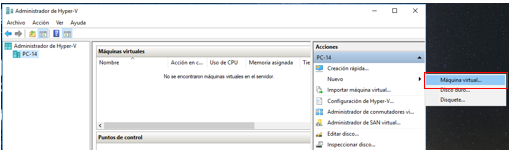
\includegraphics[width=14cm]{./Imagenes/14} 
	\end{center} 

\vspace{\baselineskip}

Nos aparece un asistente en el que nos describe algunos pasos, damos clic en “Siguiente”. 
	\begin{center}
		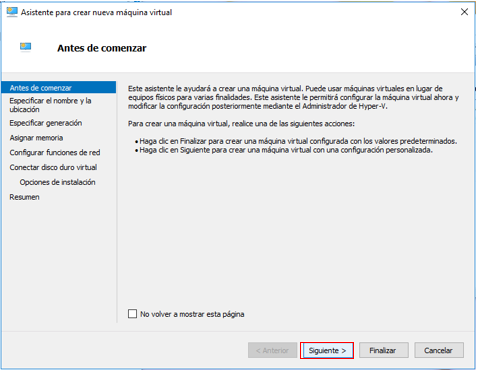
\includegraphics[width=12cm]{./Imagenes/15} 
	\end{center} 

\newpage

El segundo paso especificaremos el nombre y la ubicación, ponemos el nombre y damos clic en siguiente. 
	\begin{center}
		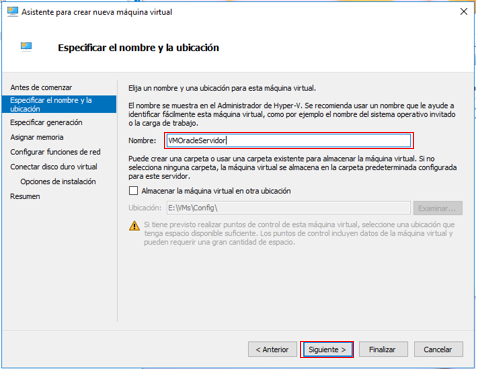
\includegraphics[width=13cm]{./Imagenes/16} 
	\end{center} 

\vspace{\baselineskip}

En esta ventana tenemos que especificar las generaciones y escogemos la opción de “Generación 1”, nos muestra una advertencia de que no se podrá cambiar su generación.  Escogemos y damos clic en “Siguiente”. 
	\begin{center}
		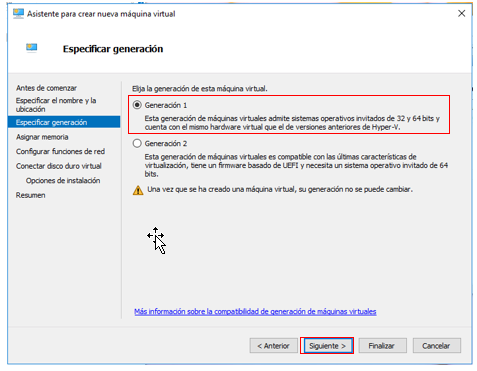
\includegraphics[width=13cm]{./Imagenes/17} 
	\end{center} 

\vspace{\baselineskip}

En esta ventana asignaremos memoria, ingresamos “2048 MB” y damos clic en “Siguiente”. 
	\begin{center}
		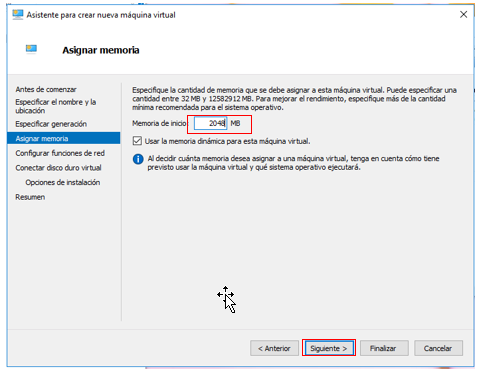
\includegraphics[width=13.2cm]{./Imagenes/18} 
	\end{center} 

\vspace{\baselineskip}

La ventana nos mostrara que tendremos que configurar funciones de red y escogemos la conexión de “AdaptadorOracle”, damos clic en “Siguiente”. 
	\begin{center}
		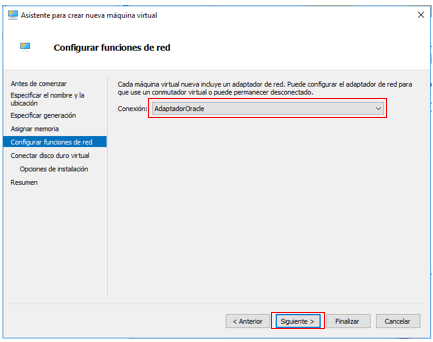
\includegraphics[width=14cm]{./Imagenes/19} 
	\end{center} 

\vspace{\baselineskip}

En esta nueva ventana tendremos un disco duro virtual, escogemos la opción de “Usar un disco duro virtual existente” y examinamos la ubicación en la se hospedará.  Damos clic en “Siguiente”.
	\begin{center}
		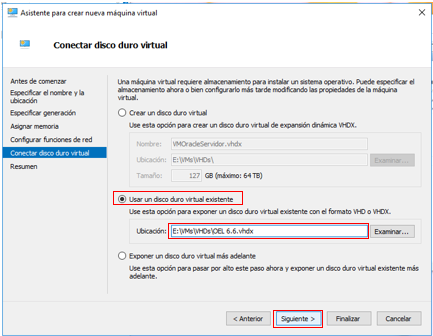
\includegraphics[width=13cm]{./Imagenes/20} 
	\end{center} 

\vspace{\baselineskip}

Como paso final nos mostrara esta pantalla el resumen de la finalización de la máquina virtual. Damos clic en “Finalizar”.
	\begin{center}
		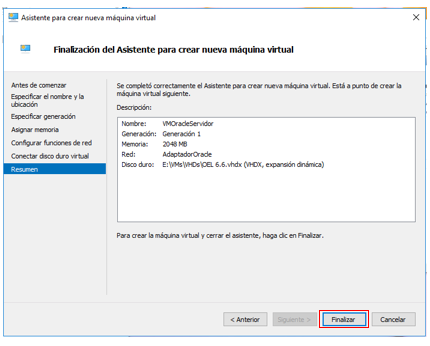
\includegraphics[width=13cm]{./Imagenes/21} 
	\end{center} 

\vspace{\baselineskip}

Veremos que se creó la máquina virtual. 
	\begin{center}
		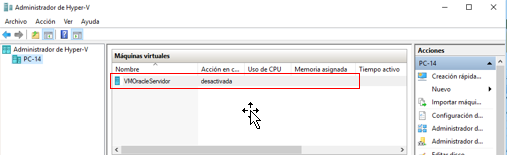
\includegraphics[width=17cm]{./Imagenes/22} 
	\end{center} 

\vspace{\baselineskip}

Ahora nos dirigimos hacia la pestaña de “Configuración”.
	\begin{center}
		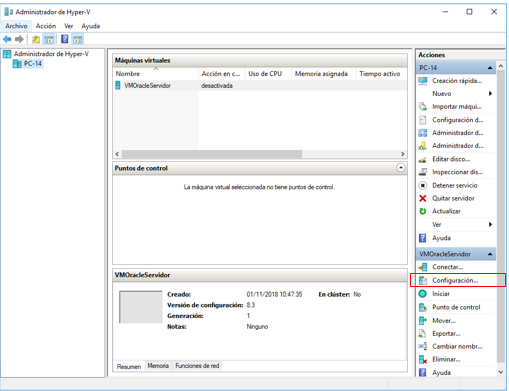
\includegraphics[width=17cm]{./Imagenes/23} 
	\end{center} 

\newpage

En la pestaña de configuraciones, cambiaremos la opción de procesador, y escogeremos a “2” el número de procesadores, y damos clic en “Aceptar”. 
	\begin{center}
		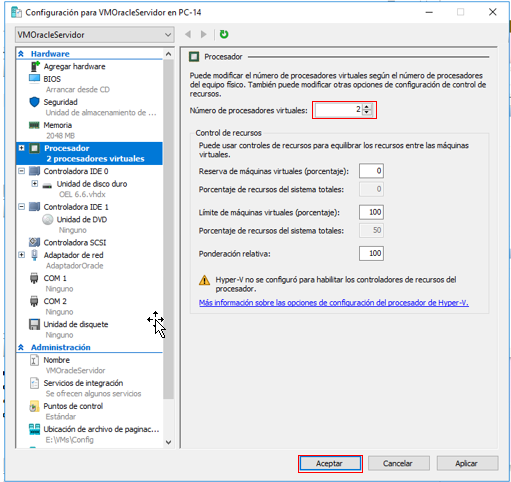
\includegraphics[width=14cm]{./Imagenes/24} 
	\end{center} 

\vspace{\baselineskip}

Ahora iniciaremos la máquina virtual, escogemos la opcion de “Iniciar”. 
	\begin{center}
		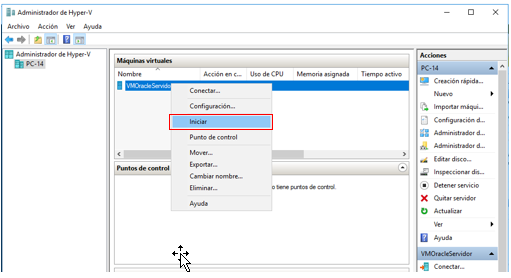
\includegraphics[width=14cm]{./Imagenes/25} 
	\end{center} 

\vspace{\baselineskip}

Ahora daremos clic en “Conectar”.
	\begin{center}
		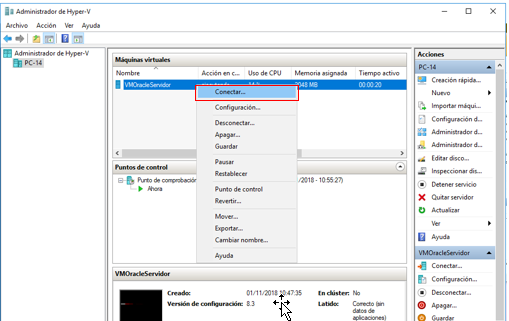
\includegraphics[width=17.5cm]{./Imagenes/26} 
	\end{center} 




\section{Desarrollo de la Actividad en la M.V.} 
\vspace{\baselineskip}
Al hacer el paso de conectar, se iniciara y podremos visualizar el usuario “Oracle” o también podremos ingresar como root. 
	\begin{center}
		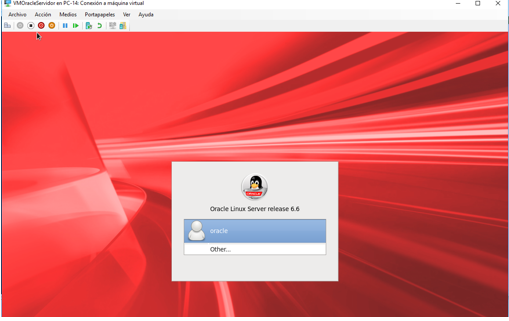
\includegraphics[width=14cm]{./Imagenes/27} 
	\end{center} 

\vspace{\baselineskip}

Nota: \\
Como usuario 2 tenemos al “oracle” y la contraseña es “oracle”. \\
Como usuario 1 tenemos a “root” y la contraseña es “oracle”, todo con minúscula. 
\\
Ingresaremos como usuario 1: root y damos clic en “Login in”.
	\begin{center}
		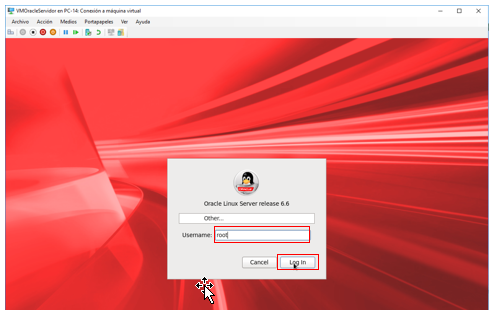
\includegraphics[width=14cm]{./Imagenes/28} 
	\end{center} 

\vspace{\baselineskip}

Ingresamos la contraseña de root “oracle”. Y damos clic en “Login in”.
	\begin{center}
		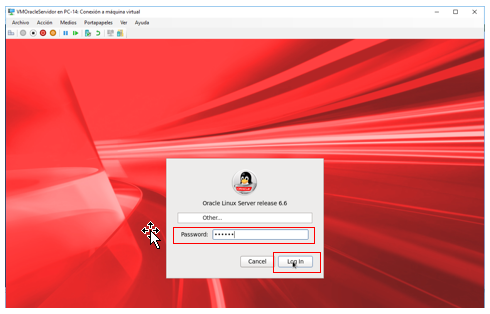
\includegraphics[width=15cm]{./Imagenes/29} 
	\end{center} 

\vspace{\baselineskip}

Ahora pasaremos a colocar una "lps": 
	\begin{center}
		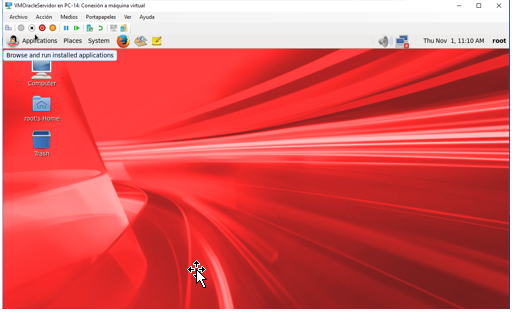
\includegraphics[width=15cm]{./Imagenes/30} 
	\end{center} 

Como vemos asi estará la estructura de la ip:
\begin{itemize}
	\item Ips: 192.168.10.x/24  *  Anfrition: 192.168.10.11  *  Huésped: 192.168.10.12
\end{itemize}

\newpage

En la maquina real vamos a la opción de “Abrir configuración de red e Internet”.
	\begin{center}
		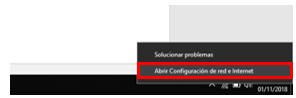
\includegraphics[width=8.6cm]{./Imagenes/31} 
	\end{center} 

\vspace{\baselineskip}

Nos mostrara esta pantalla y escogeremos la opción de “Cambiar opciones del adaptador” 
	\begin{center}
		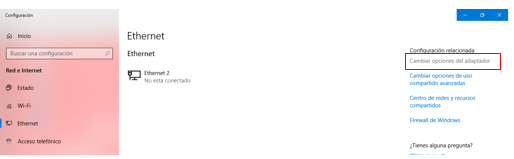
\includegraphics[width=16.5cm, height=6cm]{./Imagenes/32} 
	\end{center} 

\vspace{\baselineskip}

Tenemos que darnos cuenta en el adaptador del Hyper-v y damos clic en “Propiedades”. 
	\begin{center}
		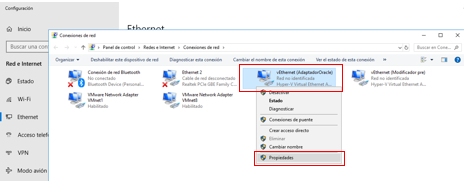
\includegraphics[width=16.5cm,height=6.8cm]{./Imagenes/33} 
	\end{center} 

\newpage

En las propiedades veremos que tendremos que ingresar una ip como muestra la imagen, una vez colocada las ip damos clic en “Aceptar”.  
	\begin{center}
		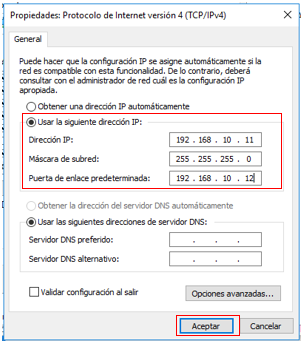
\includegraphics[width=9cm]{./Imagenes/34} 
	\end{center} 

\vspace{\baselineskip}

Ahora pasaremos a la máquina virtual donde buscaremos en la parte superior el siguiente icono y daremos clic en “Edit Connectiones …” damos clic.
	\begin{center}
		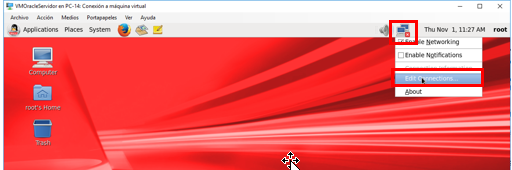
\includegraphics[width=18cm]{./Imagenes/35} 
	\end{center} 

\newpage

Se nos abrirá esta pantalla, primeramente, borraremos el que se encuentra hace años, damos clic en “Delete”.
	\begin{center}
		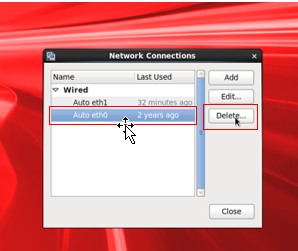
\includegraphics[width=11cm]{./Imagenes/36} 
	\end{center} 

\vspace{\baselineskip}

Ahora editaremos el único que se muestra en pantalla damos clic en “Editar”
	\begin{center}
		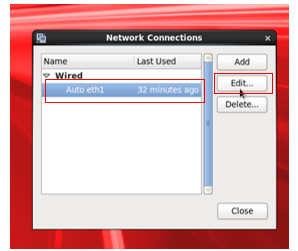
\includegraphics[width=11cm]{./Imagenes/37} 
	\end{center} 

\newpage

Nos mostrara esta ventana en el que ingresaremos la ip que colocamos de la real. Damos clic en “Aply…”.
	\begin{center}
		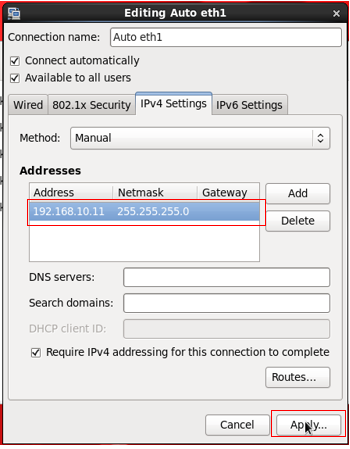
\includegraphics[width=9.5cm]{./Imagenes/38} 
	\end{center} 

\vspace{\baselineskip}

Para poder comprobar que se hizo la conexión de ethernet, abrimos el terminal de Linux, podemos hacer clic derecho en la pantalla y escoger la opción de terminal, cuando ingresemos colocamos el siguiente comando, “ping 192.198.10.11” y damos Enter, en este caso vemos que, si nos está respondiendo de manera correcta, ya que nos retorna una respuesta. 
	\begin{center}
		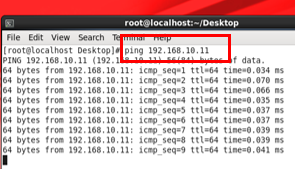
\includegraphics[width=11cm]{./Imagenes/39} 
	\end{center} 

\vspace{\baselineskip}

Como siguiente paso agregaremos el siguiente comando en la que estaremos creando una carpeta. 
	\begin{center}
		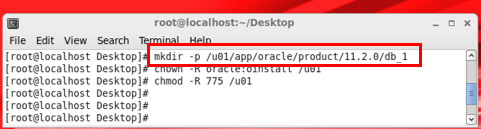
\includegraphics[width=13cm]{./Imagenes/40} 
	\end{center} 

\vspace{\baselineskip}

Luego daremos permiso con el comando “chown” que es usado para cambiar al propietario del fichero. 
	\begin{center}
		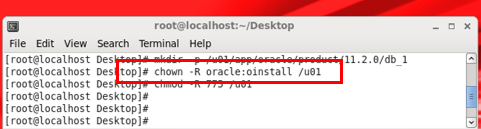
\includegraphics[width=13cm]{./Imagenes/41} 
	\end{center} 

\vspace{\baselineskip}

Daremos permiso otra vez, pero esta vez utilizaremos el comando de “chmod”, este comando permite cambiar los archivos de los permisos de acceso a los ficheros y directorios, se tiene dos métodos para realizar los cambios de permisos: 
\begin{itemize}
	\item Método nivel de control de acceso.
	\item Método octal.
\end{itemize}
Para este caso estamos utilizando el método octogonal. 
	\begin{center}
		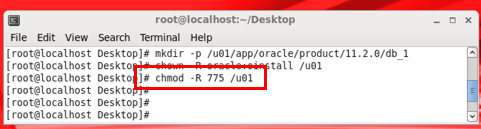
\includegraphics[width=13cm]{./Imagenes/42} 
	\end{center} 

\newpage

Como siguiente paso vamos a configurar algunos parámetros del kernel, para eso será necesario editar el archivo /etc/sysctl.conf ingresando el siguiente comando:
\begin{center}
	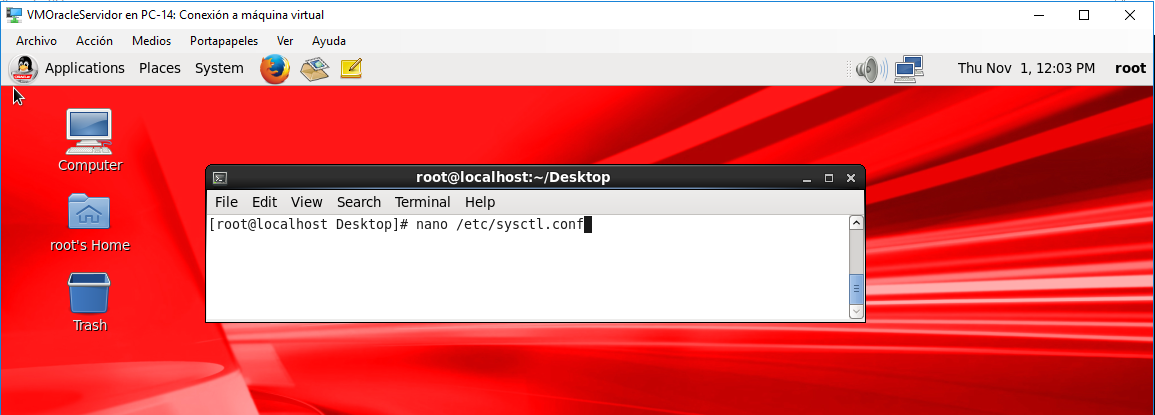
\includegraphics[width=14.35cm]{./Imagenes/43} 
\end{center} 

\vspace{\baselineskip}

Una vez dentro del archivo, añadir al final de este la siguiente información:
\begin{center}
	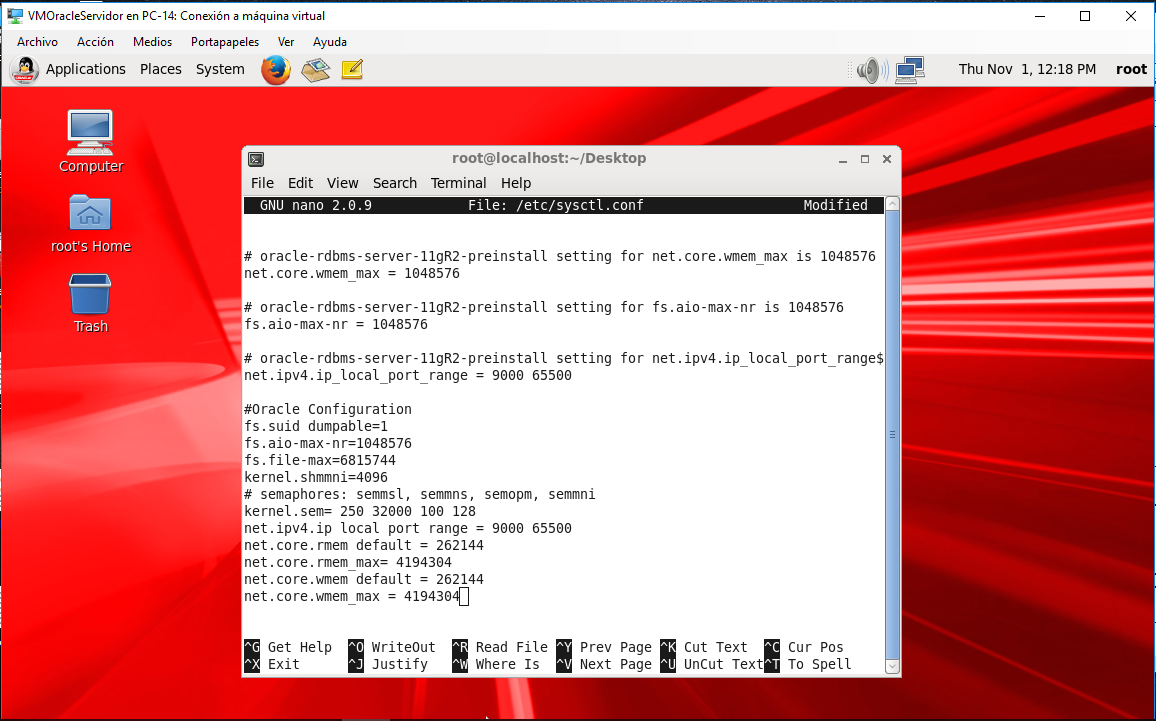
\includegraphics[width=15cm]{./Imagenes/44} 
\end{center} 

\vspace{\baselineskip}

Para salir del editor de textos presionaos la combinación de teclas (CTRL + X) y guardar los cambios. \\
Se deberá ejecutar los cambios realizados, para lo cual ejecute la siguiente sentencia en el terminal.
\begin{center}
	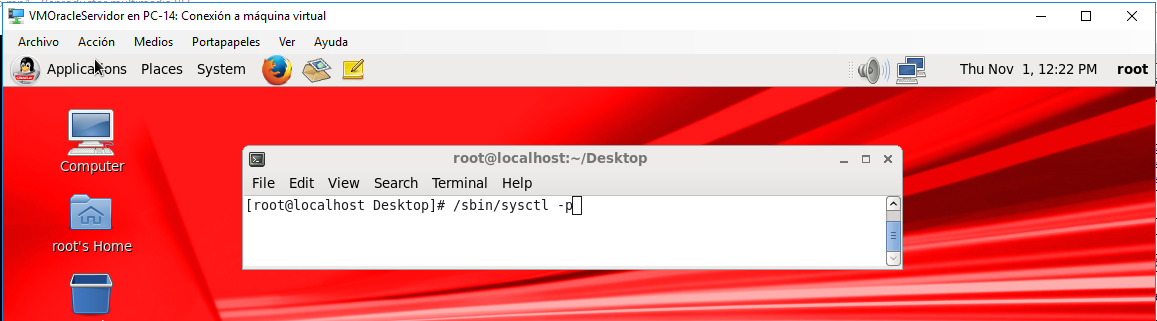
\includegraphics[width=15cm]{./Imagenes/45} 
\end{center} 

\vspace{\baselineskip}

Los resultados deberán ser similares a los siguientes:
\begin{center}
	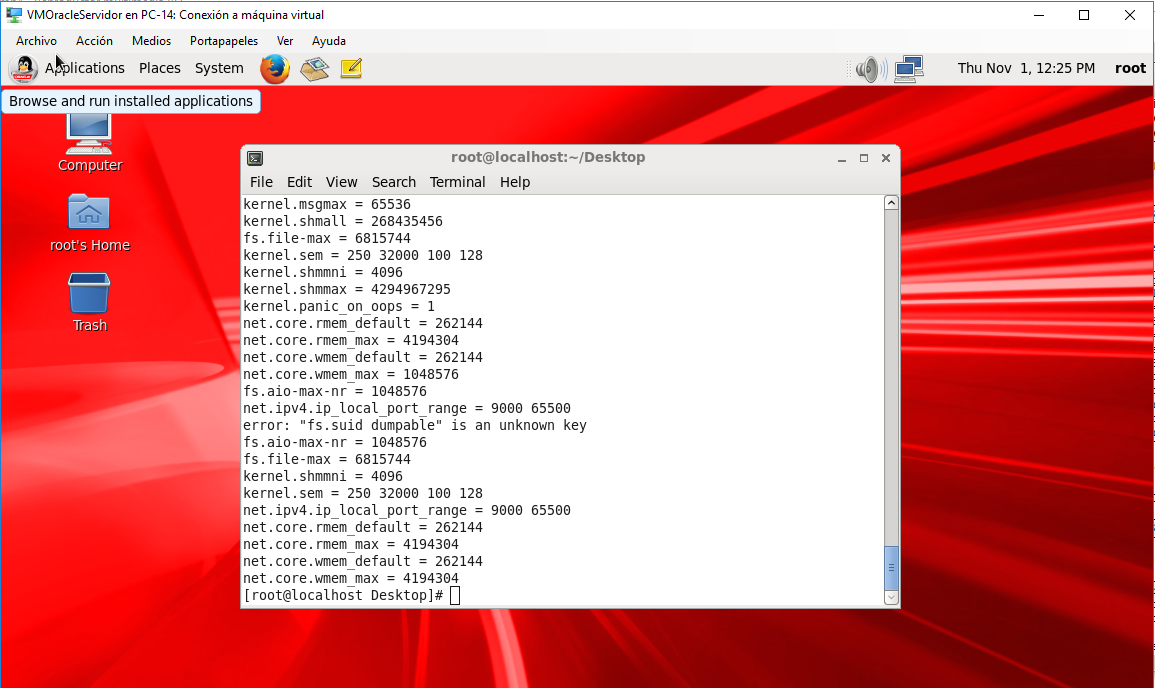
\includegraphics[width=13cm]{./Imagenes/46} 
\end{center} 

\vspace{\baselineskip}

Luego se deberá realizar cambios a los límites de seguridad del sistema para el usuario, para lo cual se debe editar el archivo /etc/security/limits.conf con el siguiente comando:
\begin{center}
	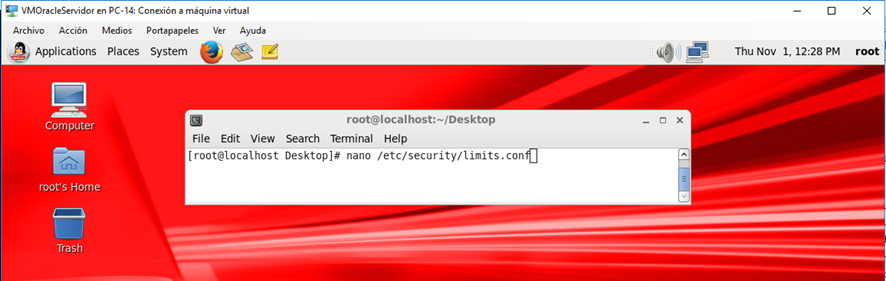
\includegraphics[width=15cm]{./Imagenes/47} 
\end{center} 

\vspace{\baselineskip}

Una vez dentro del archivo, configuramos de la siguiente manera:
\begin{center}
	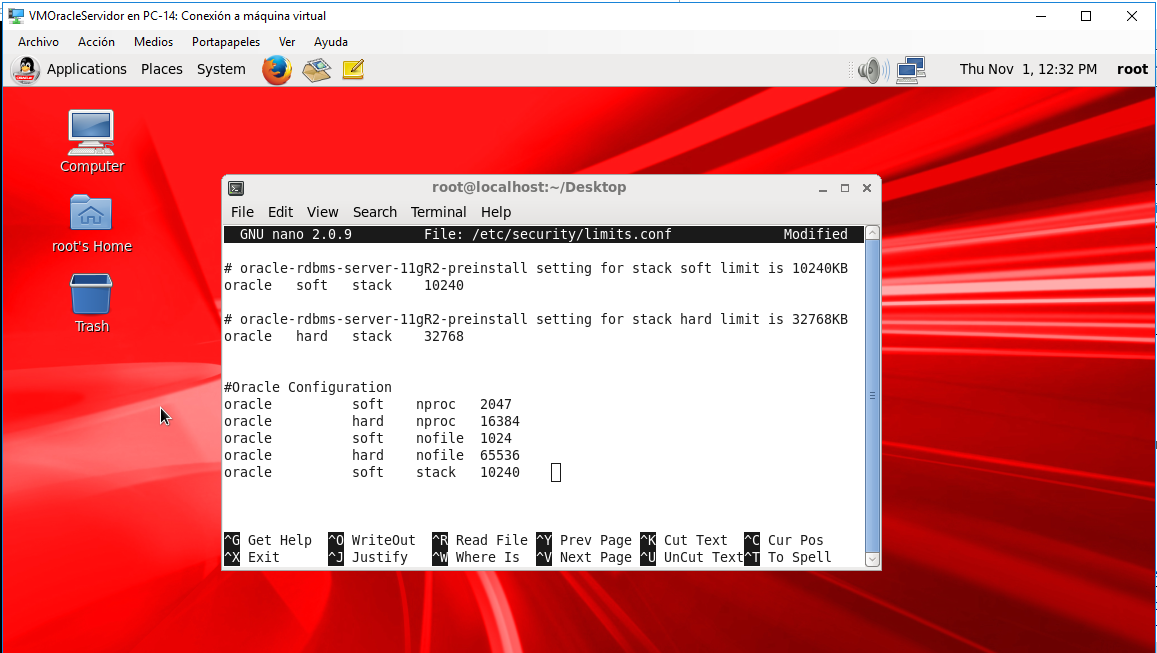
\includegraphics[width=13cm]{./Imagenes/48} 
\end{center} 

\vspace{\baselineskip}

Luego es necesario confirmar que se ha aplicado correctamente la configuración de red, para esto escribimos el siguiente comando: ifconfig eth1
\begin{center}
	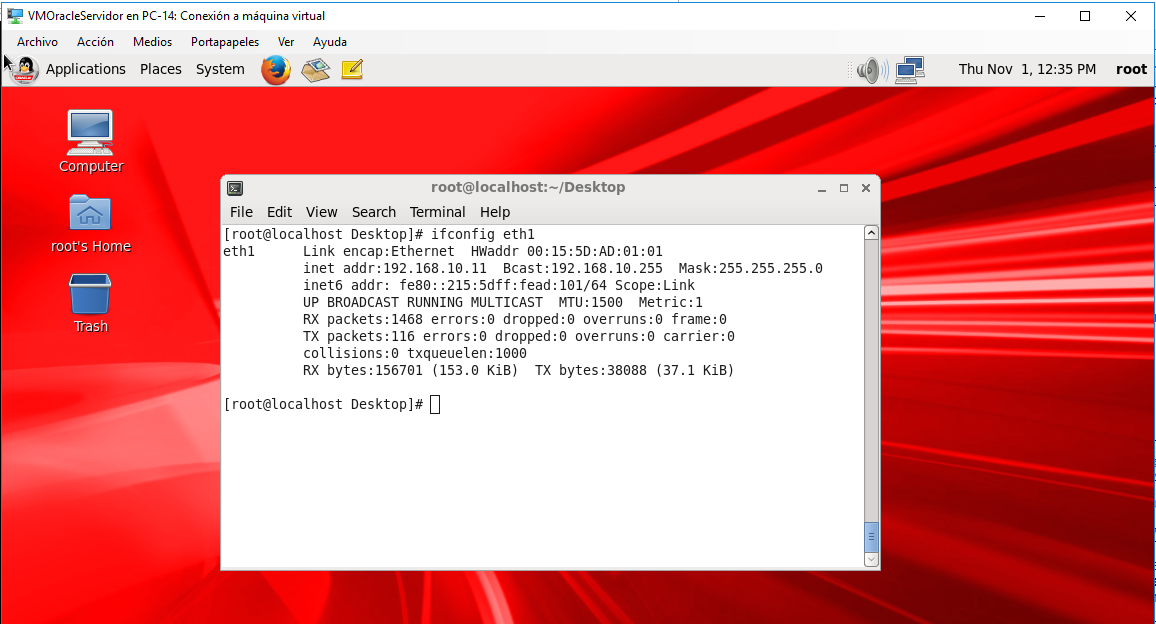
\includegraphics[width=17cm]{./Imagenes/49} 
\end{center} 

\vspace{\baselineskip}

Luego es necesario confirmar que se ha aplicado correctamente la configuración de red, para esto escribimos el siguiente comando: ifconfig eth1
\begin{center}
	\includegraphics[width=17cm]{./Imagenes/49} 
\end{center} 
El cual debe mostrarnos ese resultado.

\newpage

Luego de establecer satisfactoriamente la dirección IP de la interfaz de red, se debe configurar el nombre del servidor, para lo cual es necesario editar el archivo /etc/hosts (tener en consideración las consideraciones iniciales para establecer el nombre). Se deberá agregar el siguiente comando:
\begin{center}
	\includegraphics[width=17cm]{./Imagenes/50} 
\end{center} 

\vspace{\baselineskip}

Donde comprobaremos los datos y configuramos de la siguiente manera:
\begin{center}
	\includegraphics[width=17cm]{./Imagenes/51} 
\end{center} 
Finalmente guardar los cambios en el archivo y cerrarlo.

\vspace{\baselineskip}

Comprobamos que nuestro nombre de host sea el que ingresamos en el archivo de configuración anterior.
\begin{center}
	\includegraphics[width=17cm]{./Imagenes/52} 
\end{center} 

\vspace{\baselineskip}

A fin de terminar la configuración del sistema con el usuario “root”, es necesario reiniciar el sistema, para lo cual ingresamos el siguiente comando:
	\begin{center}
		\textbf{\large shutdown -r now}		
	\end{center}
\begin{center}
	\includegraphics[width=13cm]{./Imagenes/53} 
\end{center} 

\vspace{\baselineskip}

Esperamos a que reinicie el sistema y esta vez nos logueamos como el usuario “oracle”.
\begin{center}
	\includegraphics[width=17cm]{./Imagenes/54} 
\end{center} 

\vspace{\baselineskip}

Una vez ingresado con usuario “oracle”, ingresamos al terminal y escribimos el siguiente comando:
	\begin{center}
		\textbf{\large nano .bash profile}		
	\end{center}
\begin{center}
	\includegraphics[width=14cm]{./Imagenes/55} 
\end{center} 

\vspace{\baselineskip}

Luego ingresamos el siguiente código de configuración en el archivo abierto.
\begin{center}
	\includegraphics[width=14cm]{./Imagenes/56} 
\end{center} 

\vspace{\baselineskip}

Y volvemos a reiniciar el sistema con el siguiente comando:
\begin{center}
	\textbf{\large shutdown -r now}		
\end{center}





\end{document}
